\subsection{Veiklos modeliavimas}

Veiklos modeliavimo metodologijas galima suskirstyti pagal savybes kuriomis jos
pasižymi. Šiuo atveju jos skirstomos pagal tai, kaip naudoja žinias
%ir pagal veiklos stebėjimo padėtį.
Toks suskirstymas parodys kaip sumodeliuoti daugiau
naudingos informacijos ir kodėl šiame darbe naudojamas detalizuotas grandinės
vertės modelis (\DVCM{}).

Skirstant veiklos modeliavimo metodus pagal žinių naudojimą galima pastebėti dvi
šakas (\ref{img:business_system_modeling} pav.). Pirmoje veikla
modeliuojama naudojant patirtį iš anksčiau stebėtų veiklų, tokiu atveju
analitikas sudaro modelį, kuris jo manymu bus teisingas. Prie tokių metodologijų
galima priskirti \BPMN{} . Antroje šakoje veiklos valdymas modeliuojamas
naudojant žinias apie tai kokį modelį reikia sudaryti. Šiuo atveju yra paimamas
teorijoje aprašytas modelis ir veiklos organizuojamos pagal jį. Tuo pasižymi
\DVCM{}.

\begin{figure}[H]
	\centering
	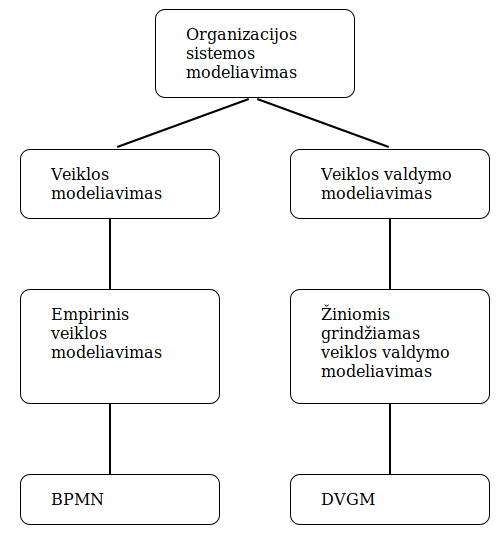
\includegraphics[width=10cm]{./sections/modeling_methods_and_languages/img/business_system_modeling}
	\caption{Veiklos modeliavimo požymiai pagal žinių naudojimą}
	\label{img:business_system_modeling}
\end{figure}

%Pagal veiklos stebėjimo padėtį metodologijas galima suskirstyti į išorinio ir
%vidinio modeliavimo. Šie būdai parodo veiklą skirtingu detalumu. Modeliuojant
%išoriniu būdu parodomos veiklos naudojimas iš išorės.


\subsection{Detalizuotas vertės grandinės modelis – DVGM} \label{section:dvcm}

\BPMN{} modelyje galima pastebėti organizacijos valdymo veiklų supratimo neapibrėžtumus \cite{bpmnPorterModel}. Taip yra todėl, kad empirinio modeliavimo metodai neparodo informacijos arba resursų transformavimo priežasčių. Tačiau įmonę galima analizuoti ir transakcinių darbų sekų modelio (\ref{img:pdca} pav.) požiūriu, tokiu būdu organizuojant veiklą kaip teoriškai teisingą.

\begin{figure}[H]
	\centering
	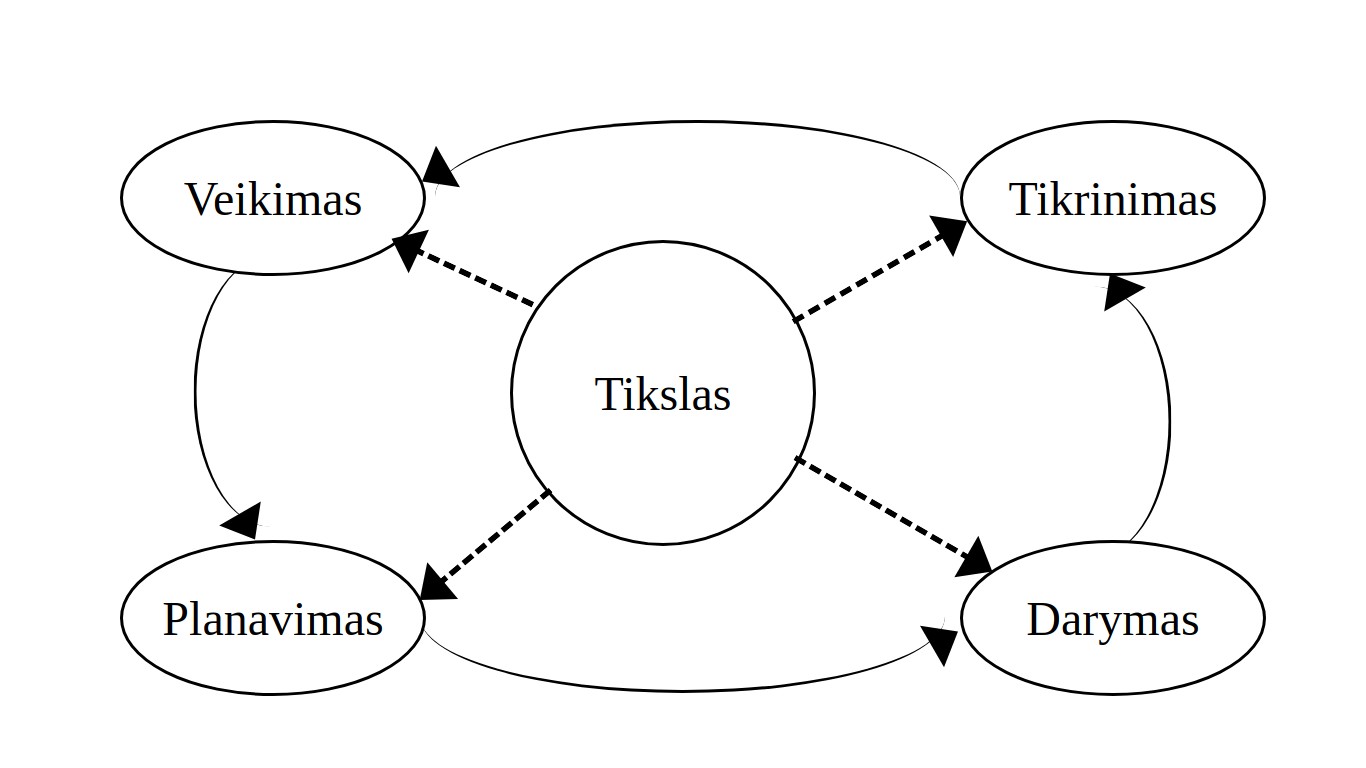
\includegraphics[width=10cm]{img/pdca}
	\caption{Transakcinių darbų sekų modelio pavyzdys}
	\label{img:pdca}
\end{figure}

Darbe organizacijos procesas bus nagrinėjamas kaip transakcijų visuma. Materialios
veiklos atskiriamos nuo valdymo veiklų. $P_i$ žymi veiklos procesą, kuris
transformuoja žaliavas, medžiagas, energiją ir formuoja materialią išeigą.
$F_j$ yra veiklos valdymo funkcija, informacijos (duomenų, žinių) transformavimo
veikla, būtina valdant procesą $P_i$. Modelis yra suskirstytas į valdymo
transakcijas $ MT_{ij} = F_j \times P_i$. Tokiu būdu pateikiama daugiau
informacijos apie įmonę. Diagrama bus vaizduojama kaip detalizuotas M.
Porterio vertės grandinės modelis (\ref{img:detalized_porter_vcm} pav).

%TODO: show goles in diagram
\begin{figure}[H]
	\centering
	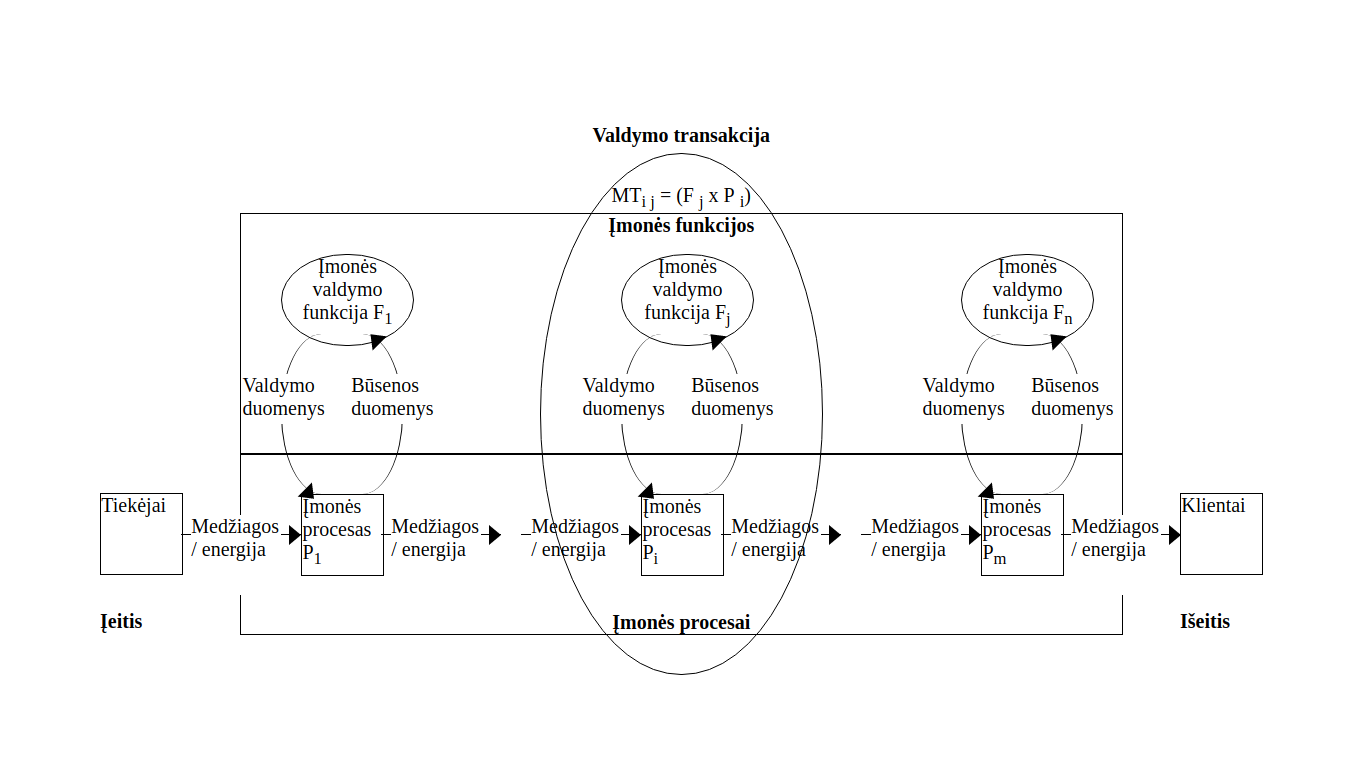
\includegraphics[height=8cm]{img/detalized_porter_vcm}
	\caption{Detalizuotas M. Porterio vertės grandinės modelis}
	\label{img:detalized_porter_vcm}
\end{figure}

Valdymo funkcija $F_j$ gali būti suskaidyta smulkiau.
(\ref{img:splitted_management_function} pav.) parodytas pavyzdys kai $F_j$
susideda iš smulkesnių dalių $F_{j1}$, $F_{j2}$ ir $F_{j3}$. Kartu visa tai
suteikia veiklos procesui $P_i$ valdymo duomenis kuriuos jis panaudoja vykdymui.
Vėliau grąžinami būsenos duomenys, jie panaudojami valdymo funkcijoje ir ciklas
kartojasi.

\begin{figure}[H]
	\centering
	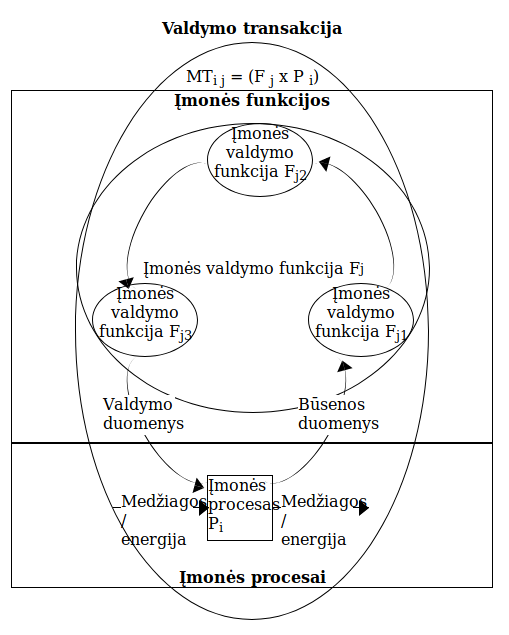
\includegraphics[width=7cm]{img/splitted_management_function}
	\caption{Valdymo funkcijos $F_j$ išskaidymo pavyzdys}
	\label{img:splitted_management_function}
\end{figure}


\subsubsection{DVGM apimtis}

Detalizuotas vertės grandinės modelis leidžia modeliuoti organizacijos veikimą kaip
transakcijų visumą. Jis atskiria vadybos veiklas nuo produkcijos veiklų.
Parodomi valdymo informacijos ciklai, kurie kontroliuoja produkcijos veiklą ir
padeda siekti organizacijos užsibrėžtų tikslų. Taip pat parodomi informacijos srautų
tipai, produkcijos veiklų įeigos ir išeigos tipai. Visa tai leidžia suprasti
kodėl įmonėje egzistuoja viena ar kita valdymo transakcija ir kaip jos įtakoja
organizacijos tikslų pasiekimą.

\subsubsection{DVGM komponentai}

Pateikiami pagrindiniai \DVCM{} komponentai. Jie leidžia veiklą modeliuoti kaip transakcinių darbų seką, kurioje procesai yra atskirti nuo valdymo funkcijų.

\begin{figure}[H]
	\centering
	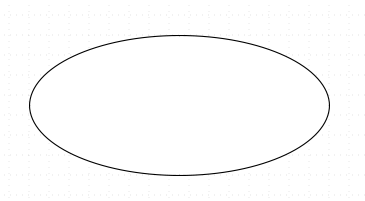
\includegraphics[height=2cm]{img/dvcm_components/management_function}
	\caption{Valdymo funkcijos žymuo}
	\label{img:dvcm_components_management_function}
\end{figure}

Valdymo funkcija (management function) darbas atliekamas organizacijoje, kuris prisideda į valdymo duomenų generavimą. Šio darbo įeiga paprastai savyje turi jo valdomo veiklos proceso proceso būseną. Atlikus darbą generuojami valdymo duomenys. Žymimas ovalu viduje paliekant vietos pavadinimui (\ref{img:dvcm_components_management_function} pav.).

\begin{figure}[H]
	\centering
	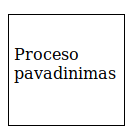
\includegraphics[height=2cm]{img/dvcm_components/process}
	\caption{Veiklos proceso žymuo}
	\label{img:dvcm_components_process}
\end{figure}

Veiklos procesas arba tiesiog procesas (process) yra darbas atliekamas organizacijoje, kuris tiesiogiai prisideda prie organizacijos gaminamos išeigos
sukūrimo. Šis komponentas valdomas valdymo funkcijų per valdymo transakcijose keliaujančius duomenis. Joms, atlikęs darbą, per interakcijų sekos srautus jis pateikia savo būsenos duomenis ir gauna valdymo duomenis. Žymimas stačiakampiu viduje paliekant vietos pavadinimui (\ref{img:dvcm_components_process} pav.).

\begin{figure}[H]
	\centering
	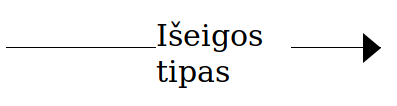
\includegraphics[height=1cm]{img/dvcm_components/sequence_flow}
	\caption{Interakcijų sekos srauto žymuo}
	\label{img:dvcm_components_sequence_flow}
\end{figure}

Interakcijų sekos srautas (interactions sequence flow) parodo valdymo funkcijų ir veiklos procesų seką, taip pat kas pagaminama atliekant darbus. Kadangi organizacijos veikla vaizduojama ciklais vieno darbo išeiga tampa kito įeiga. Šis komponentas vaizduojamas solidžia linija su užpildyto trikampio formos rodykle
gale ir išeigos (kuri tampa įeiga) tipo vardu prie pavaizduotos linijos (\ref{img:dvcm_components_sequence_flow} pav.).

\begin{figure}[H]
	\centering
	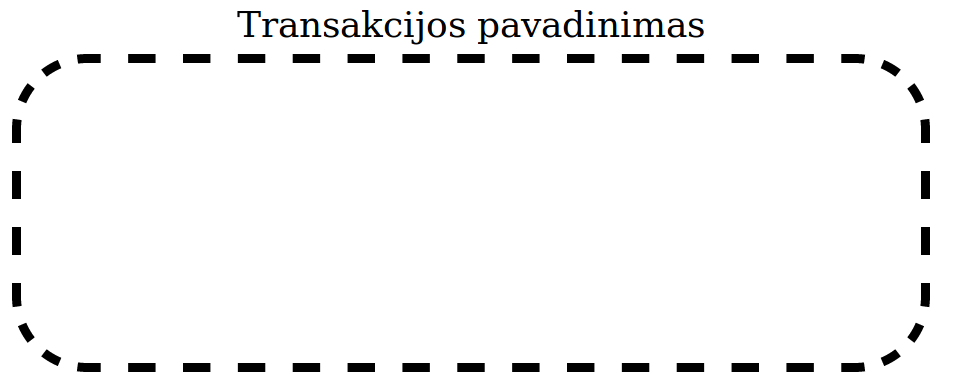
\includegraphics[height=2cm]{img/dvcm_components/management_transaction}
	\caption{Valdymo transakcijos žymuo}
	\label{img:dvcm_components_management_transaction}
\end{figure}

Valdymo transakcija (management transaction) parodo, kaip valdymo funkcijos kontroliuoja veiklos procesą. Šis komponentas žymi valdymo duomenų transformacijų ciklą. Jis vaizduojamas punktyrine linija apibraukiant transakcijai priklausantį veiklos procesą ir valdymo funkciją bei parašant transakcijos pavadinimą
(\ref{img:dvcm_components_management_transaction} pav.).

\subsubsection{DVGM komponentų tarpusavio ryšiai}

\DVCM{} komponentų tarpusavio ryšiai pavaizduoti metamodeliu (\ref{img:dvcm_metamodel} pav.). Šakninis komponentas DVGM savyje laiko valdymo transakcijas, interakcijų sekos srautus ir veiklas. Veiklos jungiamos interakcijų sekos srautais, jie taip pat nurodo kokią išeigą šiai interakcijai generuoja veikla. Veiklos skirstomos į veiklos procesus ir valdymo funkcijas. Valdymo transakcija turi nuoroda į procesą ir jį valdančią funkciją, kuri gali susidaryti iš smulkesnių dalių, taip pat sujungtų interakcijų srautais.

\begin{figure}[H]
	\centering
	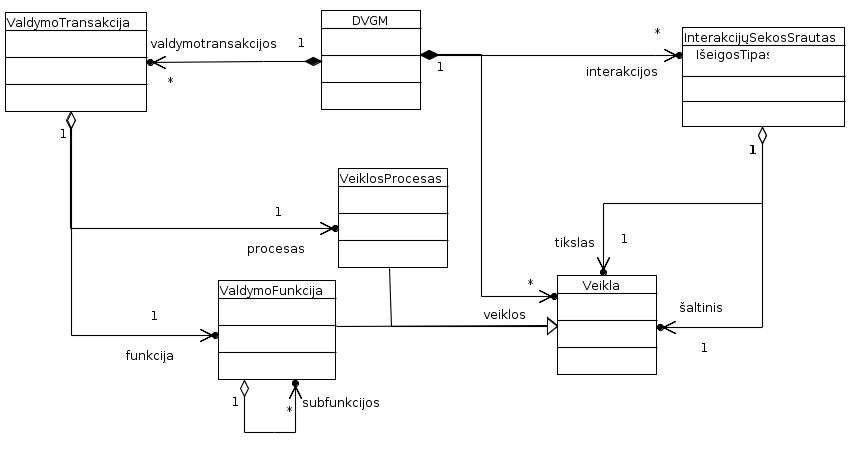
\includegraphics[width=\textwidth]{sections/modeling_methods_and_languages/img/dvcm_metamodel}
	\caption{\DVCM{} metamodelis}
	\label{img:dvcm_metamodel}
\end{figure}


\subsubsection{DVGM kaip BPMN praplėtimas}

\DVCM{} modelį galima apibrėžti ir kaip \BPMN{} praplėtimą. Paveikslas \ref{img:bpmn_extension_metamodel} vaizduoja tokį praplėtimo pavyzdį, tai bus įvesties duomenų formatas kuriamam algoritmui. Tokiu būdu apibrėžtą modelį galima nagrinėti kaip \BPMN{}.

\begin{figure}[H]
	\centering
	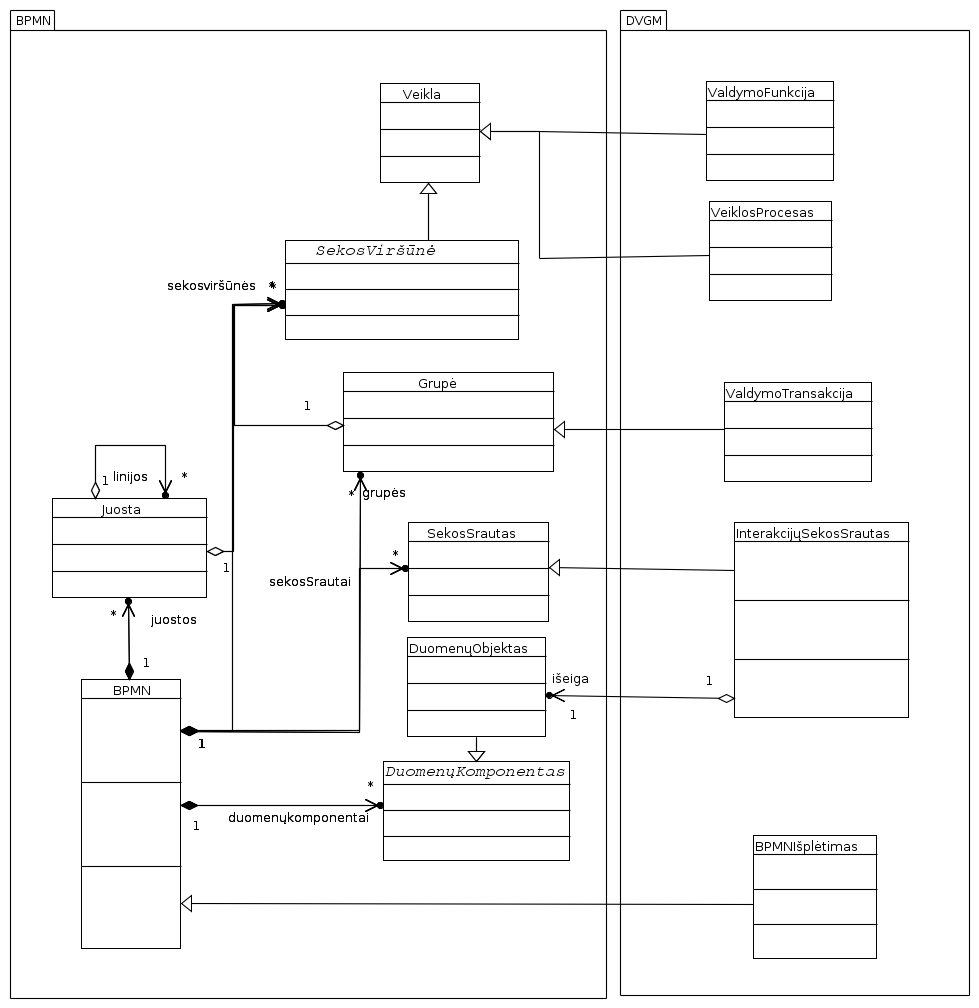
\includegraphics[width=\textwidth]{sections/modeling_methods_and_languages/img/bpmn_extension_metamodel}
	\caption{\DVCM{} kaip \BPMN{} praplėtimo metamodelis}
	\label{img:bpmn_extension_metamodel}
\end{figure}

\ref{img:bpmn_extension_metamodel} paveiksle \BPMN{} komponentai vaizduojami iš kairės, iš dešinės yra komponentai išplečiantys modelį. Veikla išplečiama valdymo funkcija ir veiklos procesu. Valdymo transakcija yra grupė, o interakcijų srautas rodo veiklų sekos srautą ir jų perduodamus duomenis. Visa Tai sudaro \BPMN{} išplėtimą.
